\pagestyle{fancy}

\fancyhf{}

\fancyhead[C]{Metodologia}
\fancyfoot[C]{\thepage}

\fancypagestyle{plain}{
    \fancyhf{}
    \fancyfoot[C]{\thepage}
}

\chapter{Metodologia}

\large

In questo capitolo, viene esposta la metodologia adottata, partendo dalle tecnologie impiegate nello sviluppo del progetto fino ai metodi di machine learning utilizzati per apprendere e valutare i risultati.

\section{Sviluppo del progetto}

\begin{table}[t]
    \centering
    \begin{tabular}{|ll|}
        \hline
        \textbf{Libreria}
        & \textbf{Descrizione} \\
        \hline
        \texttt{numpy}
        & Utilizzata per calcoli numerici avanzati. \\
        \texttt{scipy}
        & Estende numpy per il calcolo scientifico più complesso. \\
        \texttt{pandas}
        & Specializzata nella manipolazione e nell'analisi dei dati. \\
        \texttt{matplotlib}
        & Dedicata alla generazione di grafici e visualizzazioni dati. \\
        \texttt{scikit-learn}
        & Fornisce strumenti per l'apprendimento automatico. \\
        \hline
    \end{tabular}
    \caption{Panoramica delle principali librerie Python utilizzate in ambito scientifico e di data science.}
    \label{tab:5-1}
\end{table}

Come editor di codice, è stato utilizzato Visual Studio Code, noto per la sua efficienza e flessibilità, supporta molti linguaggi di programmazione ed estensioni.

\bigskip

È stato impiegata anche Jupyter, un'applicazione web open source che facilita la creazione e la condivisione di documenti con codice eseguibile, equazioni, grafici e testo.

\bigskip

È stato utilizzato GitHub, un ambiente basato su Git, che facilita la gestione del codice e la collaborazione nello sviluppo software. È possibile esaminare il progetto direttamente su \href{https://github.com/robertovicario/BSc-Computer-Science-Thesis.git}{\underline{GitHub}}. È possibile visualizzare un riassunto del codice sorgente da un notebook del progetto direttamente da \href{https://www.kaggle.com/code/robertovicario/swell-kw-stress-detection}{\underline{Kaggle}}.

\bigskip

Per la programmazione, è stato scelto Python, per la sua versatilità e l'ampio utilizzo nello sviluppo software per l'analisi dati e l'intelligenza artificiale. Sono state integrate diverse librerie di Python, evidenziate nella tabella \ref{tab:5-1}, per l'implementazione di algoritmi complessi.

\bigskip

Particolare attenzione è stata data alla libreria \texttt{scikit-learn} per la sua ampia offerta di algoritmi per classificazione, regressione, clustering e altre attività di machine learning. Per illustrare la metodologia, vengono spiegati diversi concetti che sono trattati con chiarezza nello studio \textit{"Machine learning made easy: a review of scikit-learn package in python programming language"} di Hao et al. (2019) \cite{hao2019machine}.

\section{Preprocessing dei dati}

Prima di procedere con l'addestramento dei modelli, sono state utilizzate diverse tecniche di preprocessing al fine di preparare i dati nel modo più appropriato per l'input dei modelli.

\subsection{Analisi dei dati}

Inizialmente, sono state eseguite alcune operazioni fondamentali per affrontare le sfide iniziali. Queste operazioni preliminari hanno incluso la gestione dei valori nulli nei dati, la conversione delle variabili categoriche in formati numerici e la selezione delle features più importanti. Tali passaggi sono stati eseguiti per preparare i dati in modo ottimale prima di procedere con l'addestramento dei modelli.

\subsection{Standardizzazione}

Successivamente, è stata applicata la standardizzazione che consiste nel rendere tutte le variabili comparabili tra loro, portandole a una scala comune con media zero e deviazione standard uno. In pratica, per ogni variabile, si sottrae la media della variabile e si divide per la deviazione standard della stessa.

\subsection{Principal Component Analysis}

Infine, è stata utilizzata la PCA (Principal Component Analysis), una metodologia di riduzione della dimensione utilizzata per semplificare il dataset mantenendo al contempo le informazioni più rilevanti. L'obiettivo della PCA è quello di trovare un insieme di nuove variabili, chiamate componenti principali, che sono combinazioni lineari delle variabili originali e catturano la massima varianza nei dati. È utile per eliminare la collinearità tra le variabili e per identificare le relazioni nascoste nei dati.

\section{Supervised learning}

Per presentare le metodologie e i modelli di machine learning che sono stati utilizzati, è stato fatto riferimento principalmente a due documenti. Il primo testo è \textit{"A primer on machine learning"} di Edwards et al. (2021) \cite{edwards2021primer} e il secondo è il cheatsheet \textit{"Super VIP Cheatsheet: Machine Learning"} di Amidi et al. (2019) \cite{amidi2018super}.

\bigskip

Considerando un insieme di dati composto da punti \( \mathcal{X} = \{ x_n \}_{n \in \mathbb{N}} \) e corrispondenti risultati \( \mathcal{Y} = \{ y_n \}_{n \in \mathbb{N}} \), l'obiettivo è sviluppare un modello che impari a prevedere \( \mathcal{Y} \) in funzione di \( \mathcal{X} \), ossia calcolare \( \Pr(\mathcal{Y}|\mathcal{X}) \).

\bigskip

In particolare, nell'apprendimento supervisionato si distinguono due principali metodologie:

\begin{itemize}
    \item \textbf{Classificazione}: Si occupa di assegnare una label \( y \in \mathcal{Y} \) a un dato input \( x \in \mathcal{X} \) in base a un insieme di classi predefinite \( \mathcal{X} \).
    \item \textbf{Regressione}: Ha l'obiettivo di stimare una relazione funzionale tra \( x \) e \( y \), ossia \( f: \mathcal{X} \to \mathcal{Y} \), in modo da poter fare previsioni su \( y \) per nuovi dati \( x \).
\end{itemize}

Inoltre, i modelli utilizzati in questo ambito possono essere categorizzati in due macro-categorie:

\begin{itemize}
    \item \textbf{Discriminativi}: Si concentrano sull'apprendimento della differenza tra classi, cioè stimano direttamente \( \Pr(y|x) \).
    \item \textbf{Generativi}: Propongono di generare nuovi dati che assomiglino a quelli presenti nel training set, cioè stimano \( \Pr(x|y) \) per dedurre \( \Pr(y|x) \).
\end{itemize}

\subsection{Logistic regression}

\begin{figure}[t]
    \begin{multicols}{2}
        \centering
        \includegraphics[width=\linewidth]{img//5/1.png}
        \caption{Grafico della funzione sigmoide.}
        \label{fig:5-1}
        
        \columnbreak
        
        \includegraphics[width=\linewidth]{img//5/2.png}
        \caption{Albero decisionale addestrato con dataset Iris.}
        \label{fig:5-2}
    \end{multicols}
\end{figure}

\paragraph{Funzione sigmoide}

La funzione sigmoide \( g \), conosciuta anche come funzione logistica, è definita come segue nell'equazione \ref{eq:5-1}:

\begin{equation}
    \boxed{
        \forall z \in \mathbb{R} \quad g(z) = \frac{1}{1 + e^{-z}} \in (0, 1)
    }
    \label{eq:5-1}
\end{equation}

\bigskip

La figura \ref{fig:5-1} mostra una tipica curva sigmoide.

\bigskip

Si suppone che \( y | x; \theta \) segua una distribuzione Bernoulli con parametro \( \phi \). L'equazione \ref{eq:5-2} è fondamentale per il modello di regressione logistica:

\begin{equation}
    \boxed{
        \phi = \Pr(y = 1 | x; \theta) = \frac{1}{1 + \exp{(-\theta^T x)}}
    }
    \label{eq:5-2}
\end{equation}

\subsection{Decision tree e random forest}

I modelli basati su alberi sono utilizzati per affrontare sia problemi di regressione che di classificazione. Nel progetto di tesi, sono stati utilizzati due di questi modelli:

\begin{itemize}
    \item \textbf{Decision tree}: Questo modello opera suddividendo iterativamente il dataset in base alle diverse features, con l'obiettivo di ridurre al minimo l'errore di classificazione o la deviazione nei casi di regressione. L'approccio decisionale consiste nel creare una struttura ad albero, dove ogni nodo rappresenta una decisione basata su una particolare feature, contribuendo così a delineare percorsi distinti all'interno del dataset.
    \item \textbf{Random forest}: Questo modello sfrutta un insieme di alberi decisionali. La particolarità di random forest risiede nella costruzione di ciascun albero, che avviene selezionando casualmente un sottoinsieme di features dal dataset originale. L'output finale del è ottenuto attraverso la combinazione delle previsioni di tutti gli alberi, producendo una previsione più robusta e stabile.
\end{itemize}

\bigskip

La figura \ref{fig:5-2}, mostra un albero decisionale che è stato addestrato utilizzando il famoso dataset Iris. Ogni nodo interno dell'albero corrisponde a una feature, con una condizione che divide l'insieme di dati in due. Se la condizione è vera, si passa al nodo successivo sul ramo sinistro, altrimenti si va sul ramo destro.

\section{Unsupervised learning}

L'obiettivo dell'apprendimento non supervisionato è quello di trovare modelli nascosti nei dati non etichettati \( \mathcal{X} = \{ x_n \}_{n \in \mathbb{N}} \). A differenza dell'apprendimento supervisionato, dove i dati sono etichettati con informazioni esplicite, nell'apprendimento non supervisionato non esiste alcuna guida o annotazione predefinita. Invece, l'obiettivo è identificare automaticamente schemi, gruppi o tendenze latenti all'interno dei dati stessi.

\paragraph{Clustering}

La tecnica fondamentale utilizzata nell'apprendimento non supervisionato è il clustering, che mira a raggruppare insieme dati simili in insiemi distinti, chiamati cluster, in base a determinate caratteristiche o somiglianze intrinseche tra di loro.

\paragraph{Disequazione di Jensen}

Per scoprire relazioni intrinseche tra i dati, si fa uso dei centroidi, che rappresentano i punti centrali o medi all'interno di ciascun cluster. Considerando un centroide come il valore medio \( E[\mathcal{X}] \) all'interno di ciascun cluster, è possibile applicare la disequazione di Jensen \ref{eq:5-3} per identificare relazioni tra i dati.

\begin{equation}
    \boxed{
        E[f(\mathcal{X})] \geq f(E[\mathcal{X}])
    }
    \label{eq:5-3}
\end{equation}

\bigskip

In questo progetto, è stato condotto l'addestramento di tre dei principali modelli di apprendimento non supervisionato: il k-means, il gaussian mixture, noto anche come algoritmo EM (Expectation-Maximization), e il BIRCH.

\paragraph{K-means}

\begin{figure}[t]
    \centering
    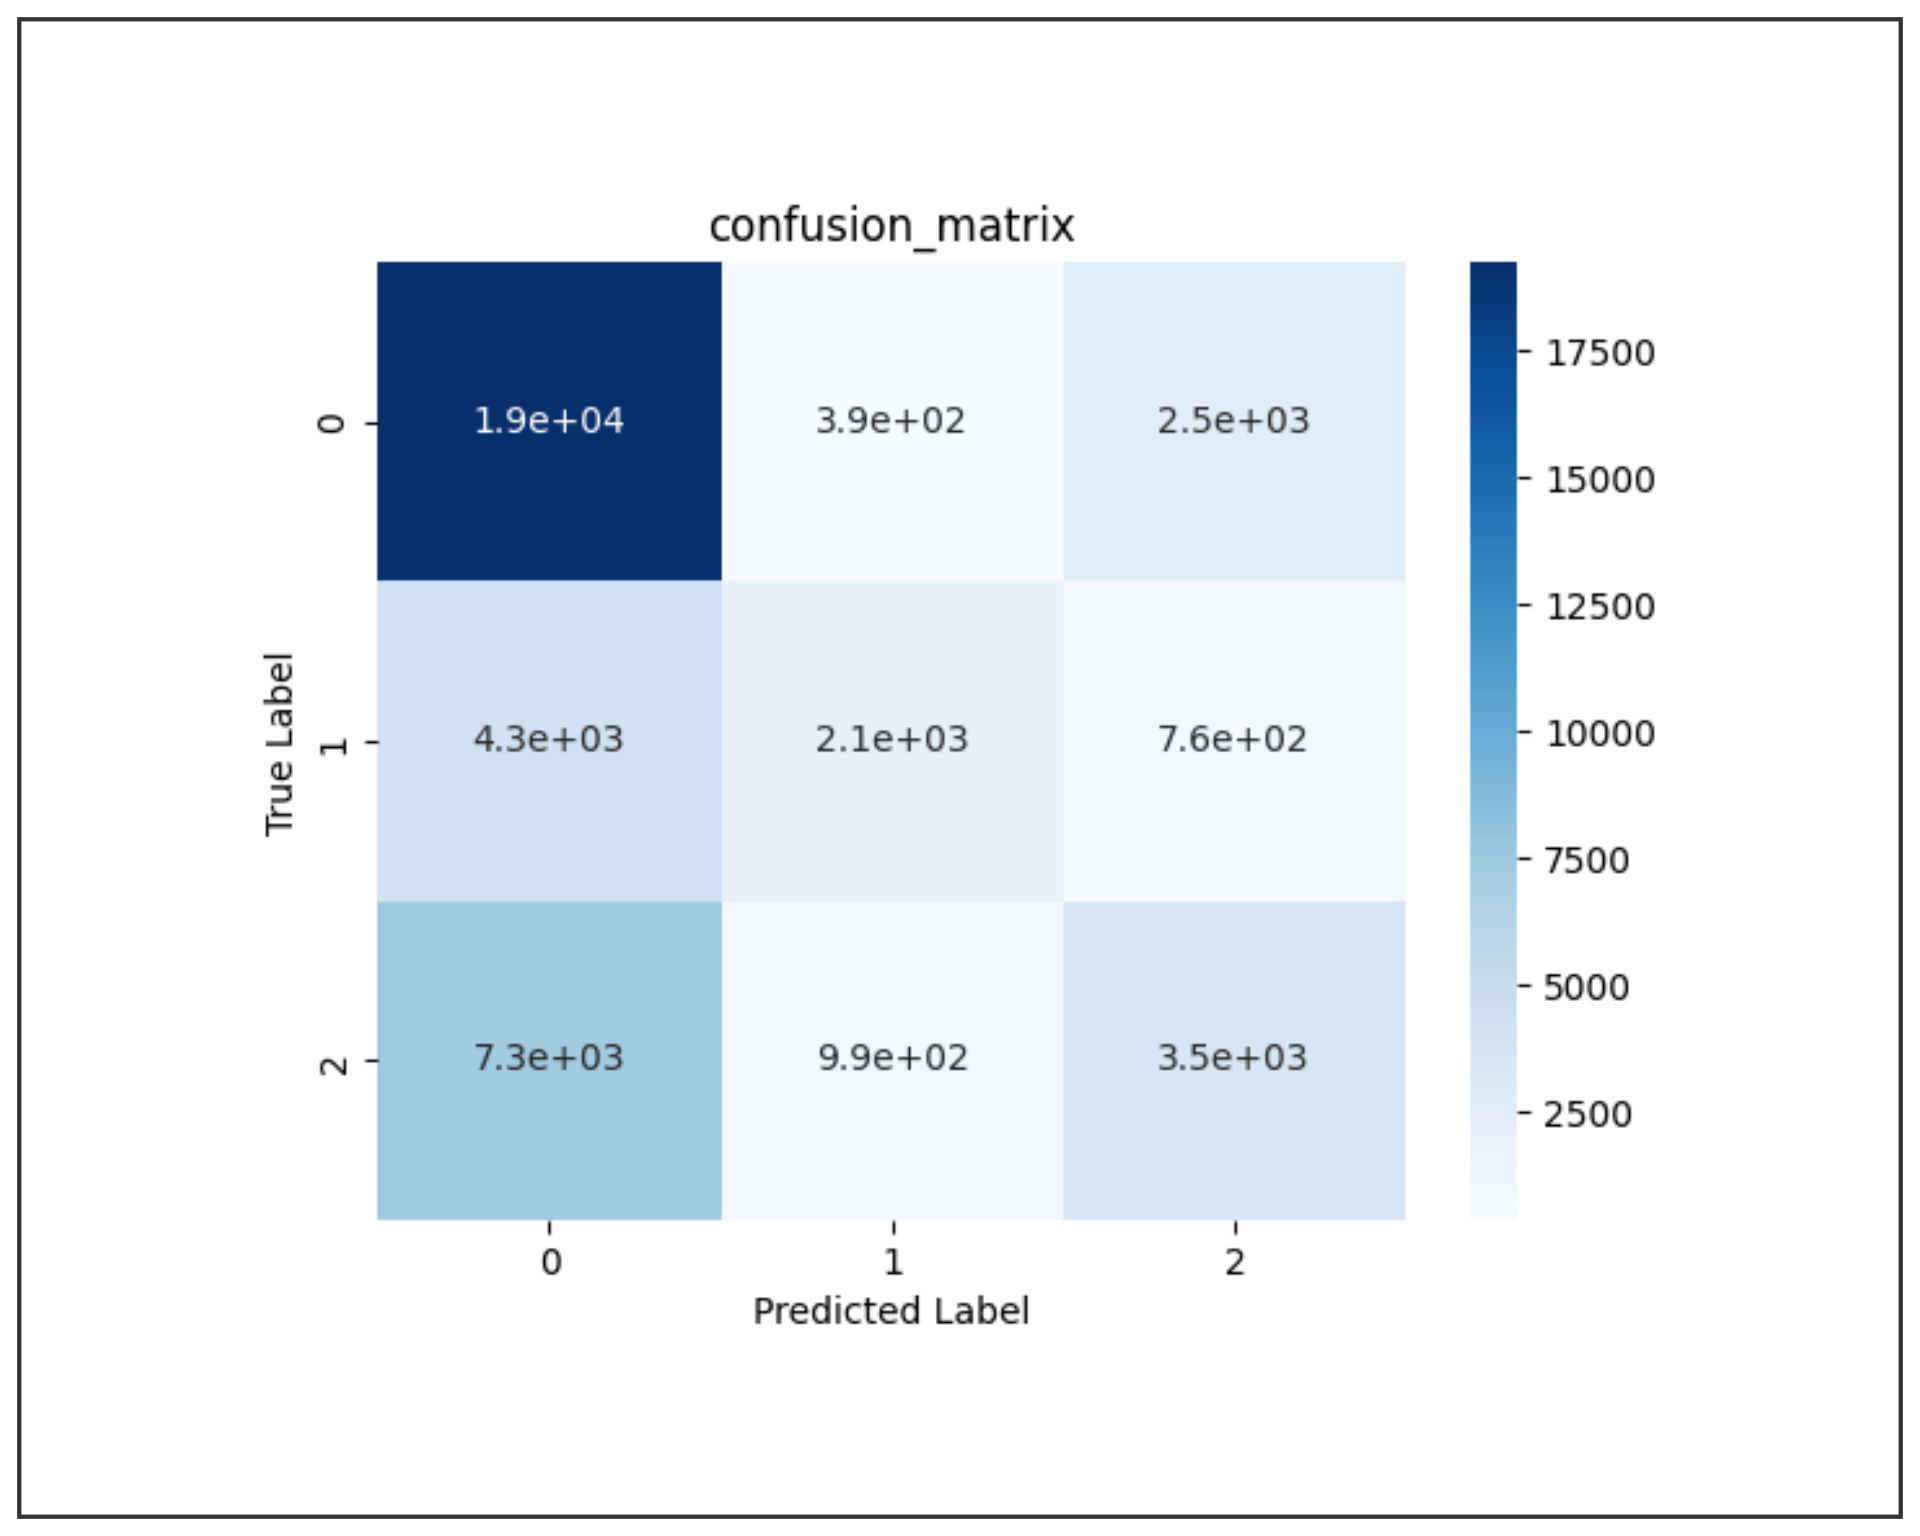
\includegraphics[width=\linewidth]{img//5/3.png}
    \caption{Processo dell'algoritmo k-means.}
    \label{fig:5-3}
\end{figure}

\begin{enumerate}
    \item Il processo inizia con l'inizializzazione dei centroidi, che sono i "means" iniziali che fungono da centro dei cluster.
    \item Successivamente, ogni punto viene assegnato al cluster del centroide più vicino.
    \item Una volta assegnati tutti i punti, la posizione dei centroidi viene aggiornata per essere il centroide (la media) di tutti i punti assegnati al cluster corrispondente.
    \item Il processo di assegnazione dei punti ai cluster e di aggiornamento dei centroidi continua fino a quando i centroidi non cambiano più la loro posizione, o cambiano molto poco, il che indica che l'algoritmo ha raggiunto la convergenza. A questo punto, si ritiene che i cluster siano stabilizzati e l'algoritmo ha completato la sua esecuzione.
\end{enumerate}

\bigskip

La figura \ref{fig:5-3}, illustra in dettaglio il processo dell'algoritmo k-means.

\paragraph{Gaussian mixture}

\begin{figure}[t]
    \centering
    \includegraphics[width=\linewidth]{img//5/4.png}
    \caption{Processo dell'algoritmo gaussian-mixture.}
    \label{fig:5-4}
\end{figure}

\begin{enumerate}
    \item Il processo inizia con l'inizializzazione delle gaussiane.
    \item Successivamente, si procede con lo step \textbf{expectation}, durante il quale ogni punto viene assegnato a una distribuzione gaussiana specifica in base alla probabilità che quel punto sia stato generato da quella distribuzione.
    \item Dopo questo step, si passa allo step di \textbf{maximization}, dove i parametri delle gaussiane vengono aggiornati in base ai punti che sono stati loro assegnati.
    \item Questi due processi continuano in modo iterativo, con i parametri delle gaussiane che vengono raffinati a ogni ciclo, fino a quando l'algoritmo non converge. A questo punto, l'algoritmo ha completato la sua esecuzione, e i cluster finali sono stabiliti insieme alle loro distribuzioni gaussiane caratteristiche.
\end{enumerate}

\bigskip

La figura \ref{fig:5-4} fornisce una rappresentazione dettagliata del procedimento dell'algoritmo gaussian mixture.

\paragraph{BIRCH}

\begin{enumerate}
    \item L'algoritmo inizia utilizzando una rappresentazione compatta dei dati nota come CF-tree per generare cluster iniziali. Questo approccio mira a ridurre la complessità computazionale durante la fase iniziale di formazione dei cluster.
    \item Successivamente, si procede con una fase di merging, in cui cluster vicini vengono combinati. Questa operazione contribuisce ulteriormente a ridurre la complessità, migliorando l'organizzazione dei dati.
    \item I passaggi di creazione iniziale e merging vengono iterati fino a raggiungere il numero desiderato di cluster o una specifica soglia di dimensioni.
\end{enumerate}

\section{Selezione del modello}

\begin{figure}[t]
    \centering
    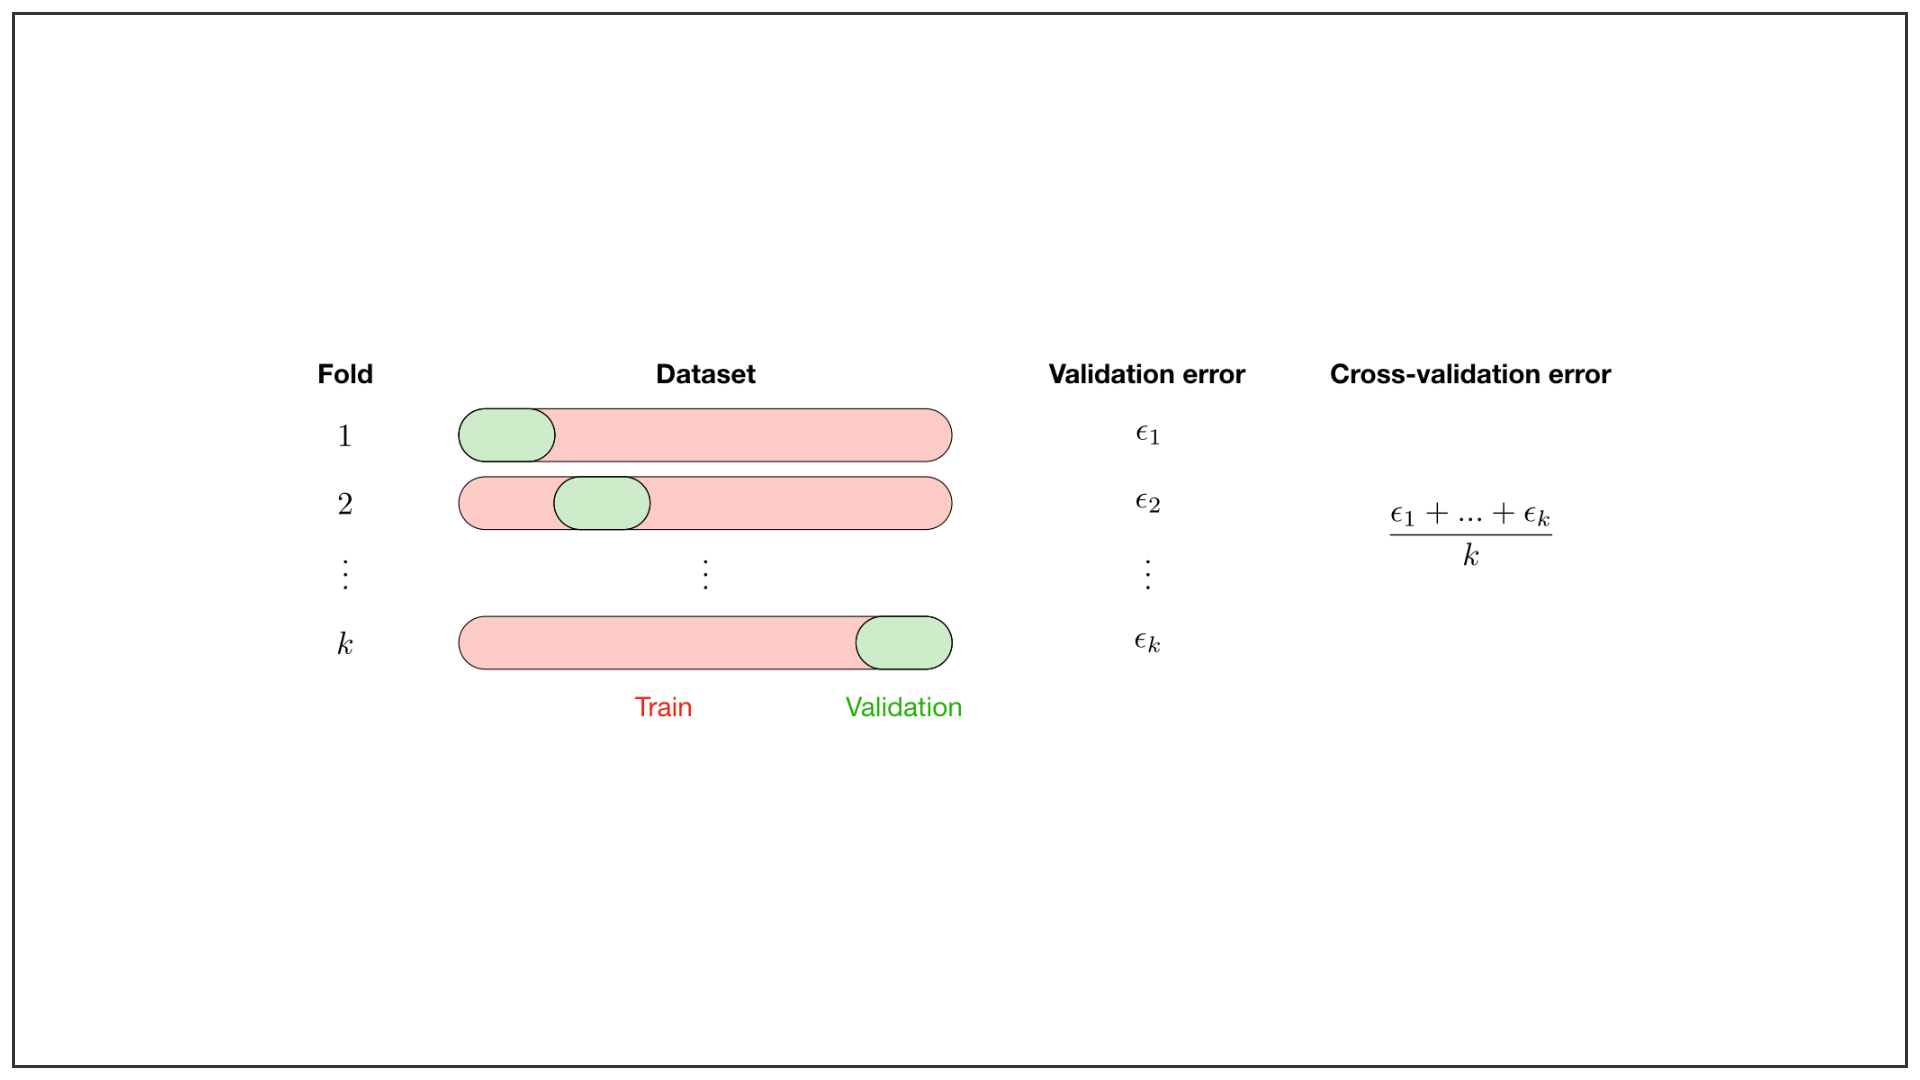
\includegraphics[width=\linewidth]{img//5/5.png}
    \caption{Esempio di k-fold cross-validation.}
    \label{fig:5-5}
\end{figure}

Prima di selezionare un modello per l'apprendimento, bisogna affrontare dinamiche fondamentali, come la capacità del modello di apprendere dai dati e la scelta degli iperparamentri. Per eseguire queste operazioni, viene suddiviso il dataset in diversi sottoinsiemi:

\begin{itemize}
    \item \textbf{Training set}: La parte di dataset destinata all'apprendimento.
    \item \textbf{Validation set}: È una porzione di dati utilizzata per valutare il modello.
    \item \textbf{Testing set}: Il sottoinsieme impiegato per le previsioni e i risultati.
\end{itemize}

\subsection{Cross-validation}

La cross-validation è una metodologia impiegata per scegliere un modello che non sia eccessivamente dipendente dal dataset di addestramento originale, ovvero dalla distribuzione dei dati del training set.

\bigskip

La figura \ref{fig:5-5}, illustra la k-fold cross-validation, una tra le possibili implementazioni di cross-validation, che è stata impiegata anche nel progetto connesso alla seguente tesi.

\paragraph{K-fold cross-validation}

\begin{enumerate}
    \item Il dataset viene suddiviso in k parti (fold) di uguali dimensioni. Per ogni fold, il modello viene addestrato sui dati di \( k-1 \) fold e validato sul fold rimanente.
    \item Questo processo è ripetuto k volte, con ogni fold utilizzato una volta come validation set.
    \item Per ogni fold, veongono registrati gli errori di validazione. L'errore di convalida è calcolato come la media degli errori di validazione dei singoli fold.
\end{enumerate}

\section{Metriche di performance}

\begin{figure}[t]
    \begin{multicols}{2}
        \centering
        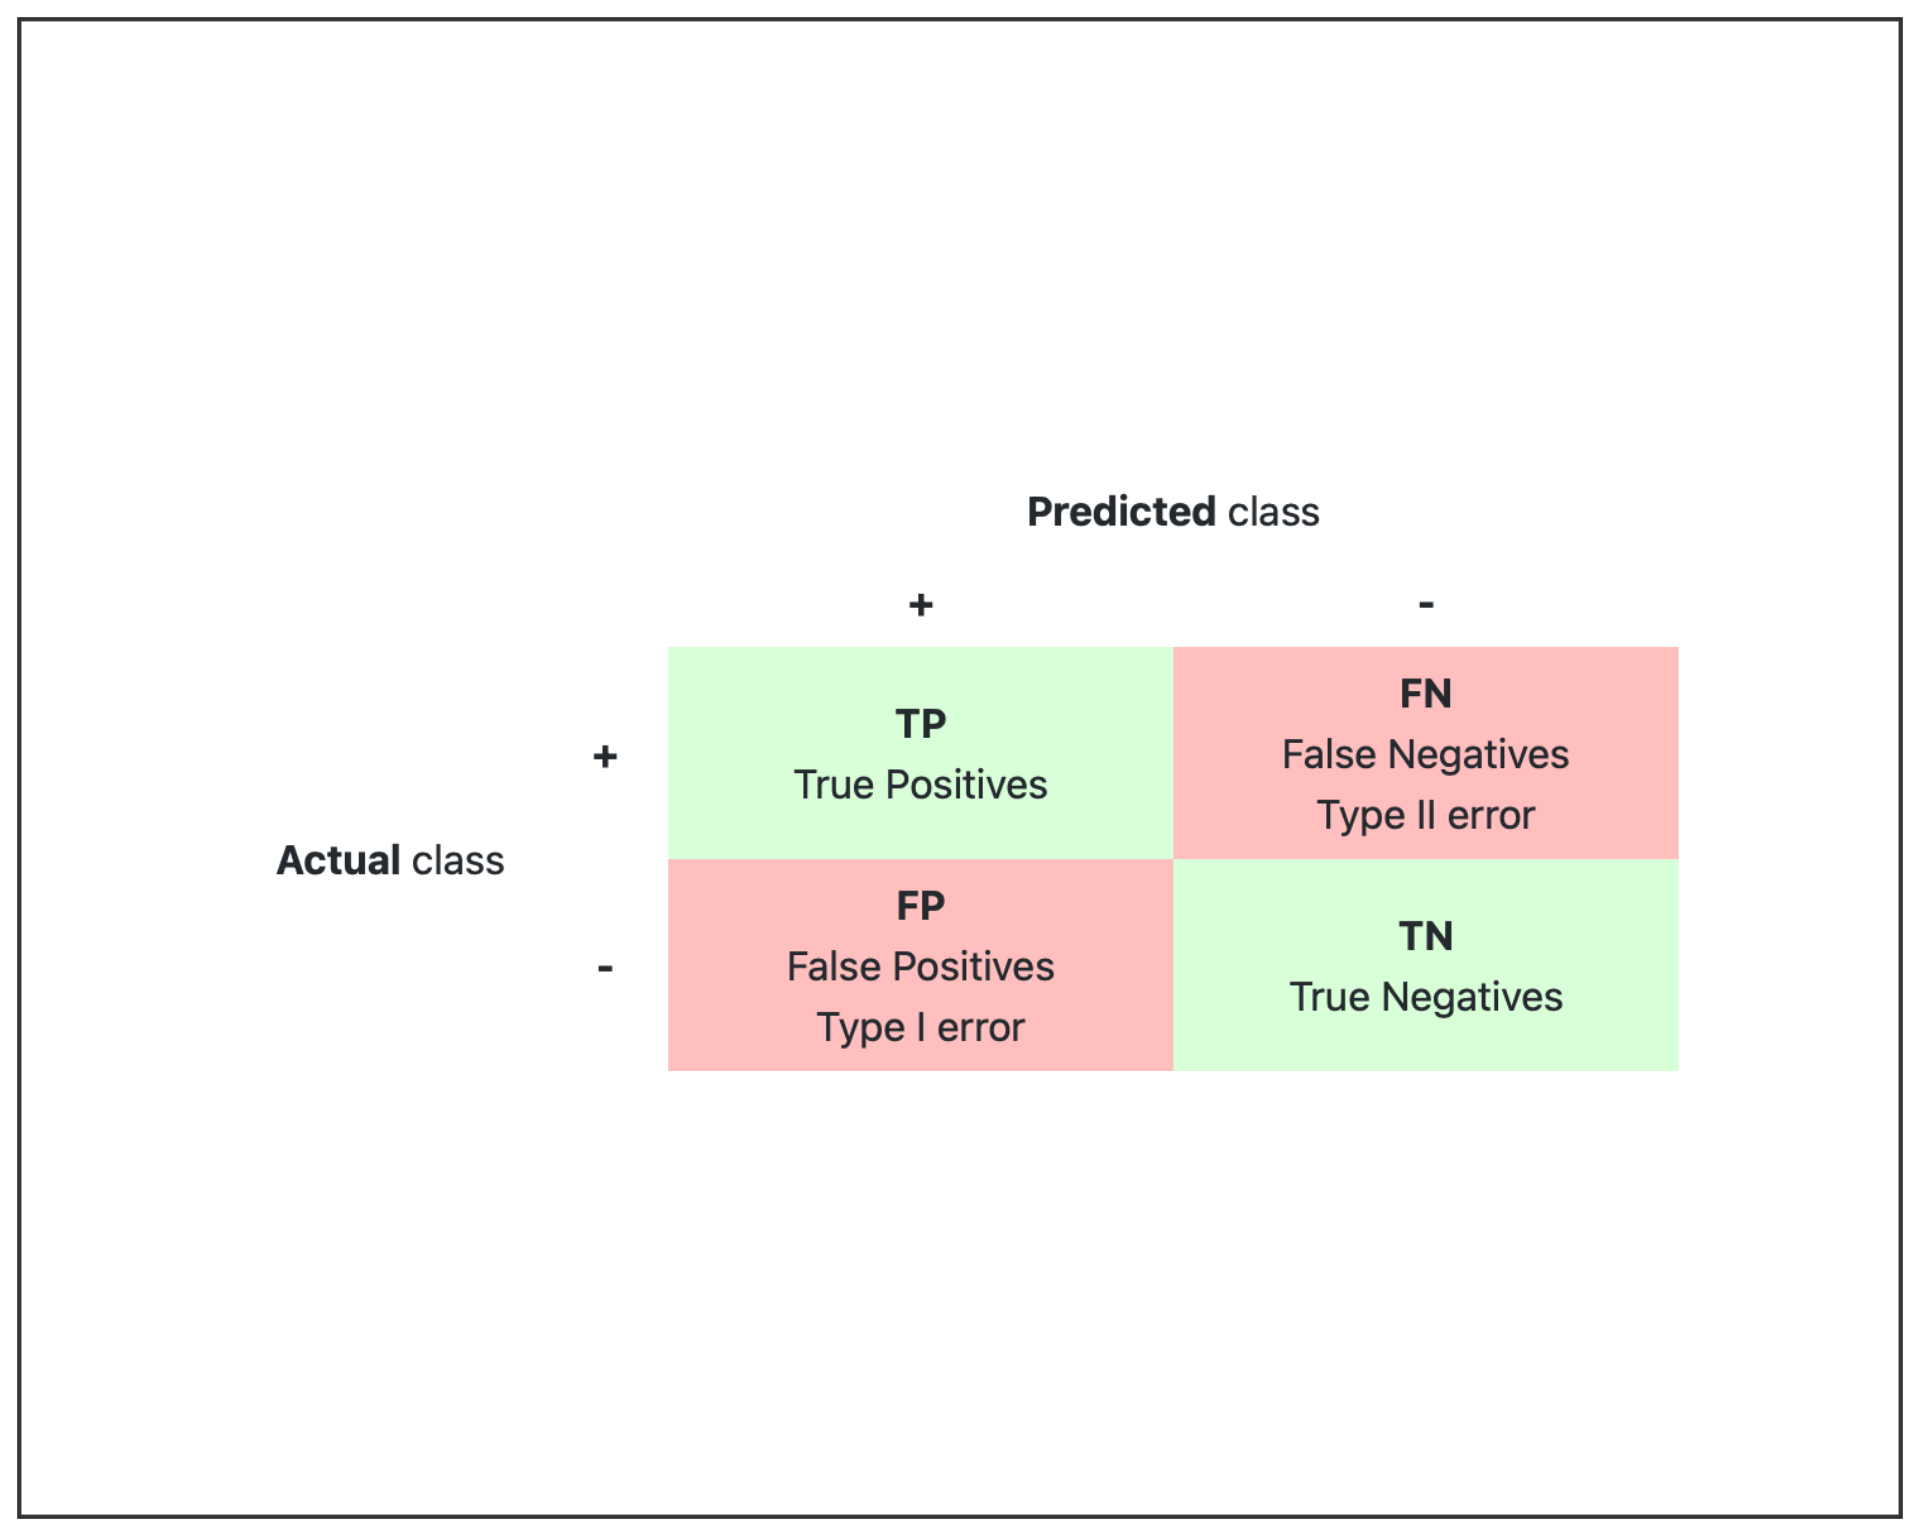
\includegraphics[width=\linewidth]{img//5/6.png}
        \caption{Matrice di confusione che illustra la classificazione binaria dei risultati di un modello predittivo.}
        \label{fig:5-6}
        
        \columnbreak
        
        \includegraphics[width=\linewidth]{img//5/7.png}
        \caption{Grafico silhouette di un clustering utilizzando il k-means.}
        \label{fig:5-7}
    \end{multicols}
\end{figure}

Per valutare in modo completo le prestazioni dei modelli, sono state impiegate diverse metriche. Queste metriche possono variare in base al tipo di modello selezionato.

\bigskip

I modelli utilizzati per la classificazione sono stati principalmente valutati utilizzando l'\textbf{accuratezza} come metrica di valutazione. L'accuratezza misura la proporzione di predizioni corrette rispetto al totale delle istanze nel dataset. L'equazione \ref{eq:5-4}, mostra la rappresentazione matematica dell'accuratezza.

\begin{equation}
    \boxed{
        \text{Accuracy} = \frac{TP + TN}{TP + TN + FP + FN}
    }
    \label{eq:5-4}
\end{equation}

\bigskip

Per ottenere una valutazione più completa delle prestazioni dei modelli di classificazione, è possibile utilizzare una \textbf{matrice di confusione}. La figura \ref{fig:5-6}, mostra la struttura di una matrice di confusione, nella quale sono riportati i risultati delle previsioni del modello rispetto alle classi effettive dei dati di test. Questa matrice è chiamata "di confusione" perché aiuta a comprendere quanto il modello possa confondersi tra le diverse classi.

\bigskip

I modelli che hanno utilizzato il clustering come tecnica di apprendimento, sono stati valutati utilizzando il \textbf{punteggio silhouette}. Questo punteggio, fornisce un'indicazione su quanto i punti dati all'interno di ogni cluster siano simili tra loro rispetto a quanto siano dissimili dai punti nei cluster adiacenti. Il punteggio silhouette varia da -1 a 1. Un punteggio positivo indica che l'oggetto è stato assegnato in modo appropriato al suo cluster, mentre un punteggio negativo indica che potrebbe essere assegnato a un cluster diverso. Un punteggio di zero suggerisce che l'oggetto è sulla soglia tra due cluster e potrebbe essere assegnato in modo ambiguo. Il calcolo di questo punteggio può essere effettuato mediante l'equazione \ref{eq:5-5}.

\begin{equation}
    \boxed{
        s = \frac{b - a}{\max(a, b)}
    }
    \label{eq:5-5}
\end{equation}

\bigskip

Dove \( a \) rappresenta la distanza media all'interno di un cluster e \( b \) rappresenta la distanza minima media tra un punto in un cluster e i punti nel cluster adiacente più vicino.

\bigskip

Per ulteriori analisi dei risultati del clustering, è stato impiegato il \textbf{grafico silhouette}. La rappresentazione di questo diagramma è visibile nella figura \ref{fig:5-7}, che aiuta a individuare la corretta definizione dei cluster e la collocazione del punteggio silhouette.